\documentclass[compress]{beamer}
\usepackage{ifthen,verbatim}

\newcommand{\isnote}{}
\xdefinecolor{lightyellow}{rgb}{1.,1.,0.25}
\xdefinecolor{darkblue}{rgb}{0.1,0.1,0.7}

%% Uncomment this to get annotations
%% \def\notes{\addtocounter{page}{-1}
%%            \renewcommand{\isnote}{*}
%% 	   \beamertemplateshadingbackground{lightyellow}{white}
%%            \begin{frame}
%%            \frametitle{Notes for the previous page (page \insertpagenumber)}
%%            \itemize}
%% \def\endnotes{\enditemize
%% 	      \end{frame}
%%               \beamertemplateshadingbackground{white}{white}
%%               \renewcommand{\isnote}{}}

%% Uncomment this to not get annotations
\def\notes{\comment}
\def\endnotes{\endcomment}

\setbeamertemplate{navigation symbols}{}
\setbeamertemplate{headline}{\mbox{ } \hfill
\begin{minipage}{5.5 cm}
\vspace{-0.75 cm} \small
\end{minipage} \hfill
\begin{minipage}{4.5 cm}
\vspace{-0.75 cm} \small
\begin{flushright}
\ifthenelse{\equal{\insertpagenumber}{1}}{}{Jim Pivarski \hspace{0.2 cm} \insertpagenumber\isnote/\pageref{numpages}}
\end{flushright}
\end{minipage}\mbox{\hspace{0.2 cm}}\includegraphics[height=1 cm]{../cmslogo} \hspace{0.1 cm} \includegraphics[height=1 cm]{../tamulogo} \hspace{0.01 cm} \vspace{-1.05 cm}}

\begin{document}
\begin{frame}
\vfill
\begin{center}
\textcolor{darkblue}{\Large Track-based alignment updates?  (No.)}

\vfill
\begin{columns}
\column{0.3\linewidth}
\begin{center}
\large
\textcolor{darkblue}{Jim Pivarski}
\end{center}
\end{columns}

\begin{columns}
\column{0.3\linewidth}
\begin{center}
\scriptsize
{\it Texas A\&M University}
\end{center}
\end{columns}

\vfill
11 December, 2009

\end{center}
\end{frame}

%% \begin{notes}
%% \item This is the annotated version of my talk.
%% \item If you want the version that I am presenting, download the one
%% labeled ``slides'' on Indico (or just ignore these yellow pages).
%% \item The annotated version is provided for extra detail and a written
%% record of comments that I intend to make orally.
%% \item Yellow notes refer to the content on the {\it previous} page.
%% \item All other slides are identical for the two versions.
%% \end{notes}

\small

\begin{frame}
\frametitle{Tracker cooling incident}

\begin{itemize}
\item Below: module position differences before and after cooling incident

\item Left: ``after'' = prompt alignment performed immediately after
  incident (low statistics, but pinpoints the motion in time)

\item Right: ``after'' = full-statistics November cosmic ray alignment
\end{itemize}

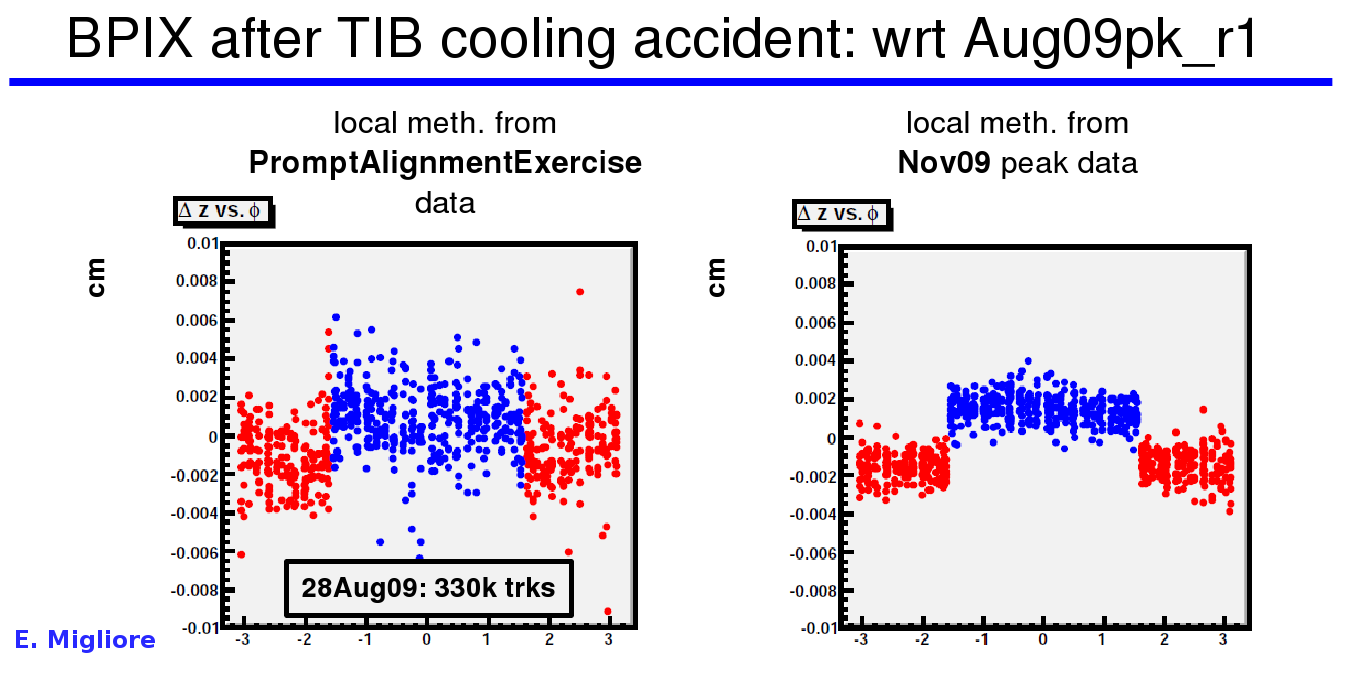
\includegraphics[width=\linewidth]{pxb_motion.png}
\end{frame}

\begin{frame}
\frametitle{New muon alignment?}

\begin{itemize}
\item Tracker alignment has been updated using post-incident
  (October-November) cosmic rays, $N_{\mbox{\scriptsize Oct-Nov}}/N_{\mbox{\scriptsize CRAFT}} \sim 2/3$
\item GlobalMuons in the same run range: most runs are empty
  (presumably, tracker and DT were not taking data concurrently, as
  they were during CRAFT)
\item Available runs for muon alignment: 118862, 118964, 118967,
  118969; $N_{\mbox{\scriptsize Oct-Nov}}/N_{\mbox{\scriptsize CRAFT}} \sim 0.25$\%
\item Only 52 chambers can be aligned, with low resolution
\item Verify that the CRAFT-09 muon alignment is consistent with the
  post-incident tracker geometry in post-incident data

(i.e.\ tracker moved, muon chambers didn't; verify that we see the
  same muon chamber positions when the right tracker description is
  used in both cases)
\end{itemize}
\end{frame}

\begin{frame}
\frametitle{Results (1/4)}
\begin{itemize}
\item Left: difference-over-statistical error, should be unit Gaussian

(blue curve is a unit Gaussian, not a fit)

\item Right: plain differences

\item Consistent within uncertainties: 0.66~mm
\end{itemize}

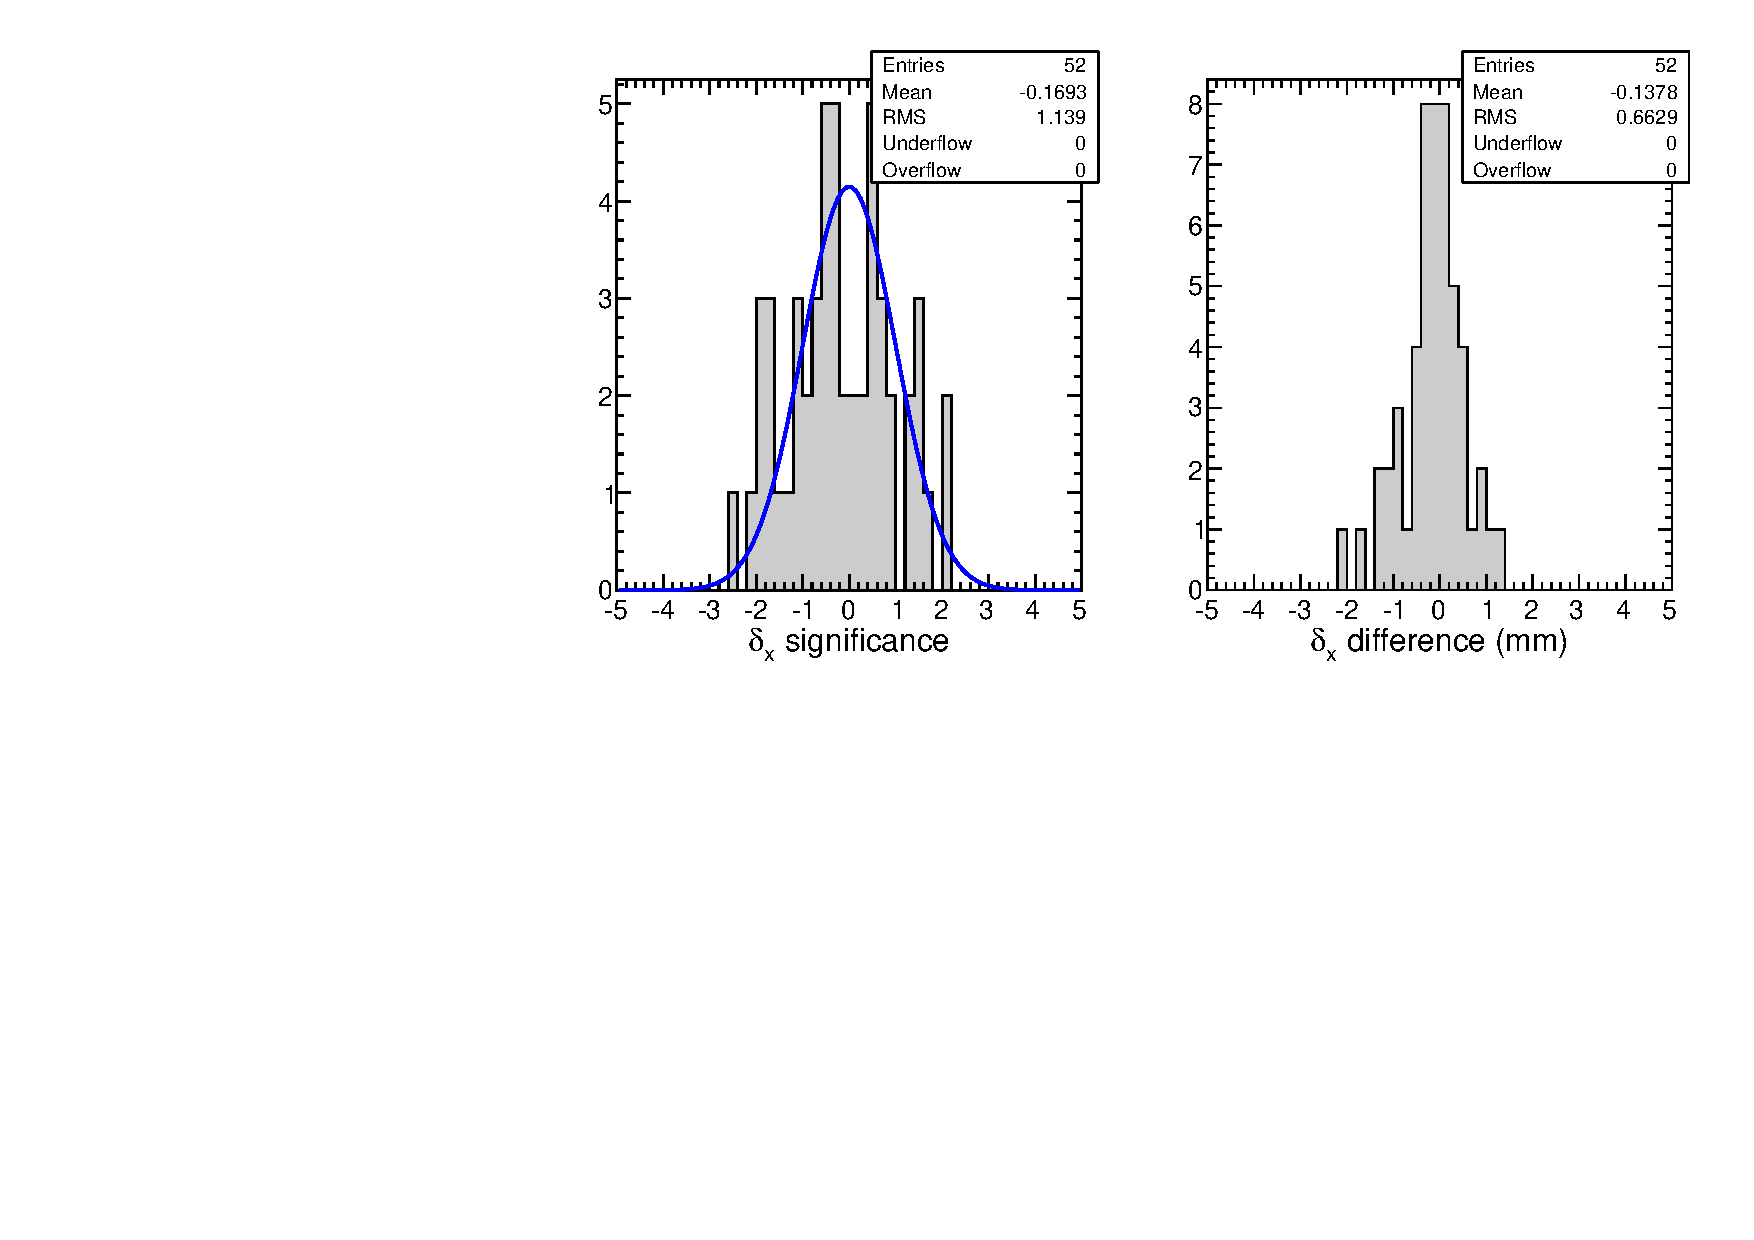
\includegraphics[width=\linewidth]{afterincident_x.pdf}
\end{frame}

\begin{frame}
\frametitle{Results (2/4)}
\begin{itemize}
\item Left: difference-over-statistical error, should be unit Gaussian

(blue curve is a unit Gaussian, not a fit)

\item Right: plain differences

\item Consistent within uncertainties: 1.2~mm
\end{itemize}

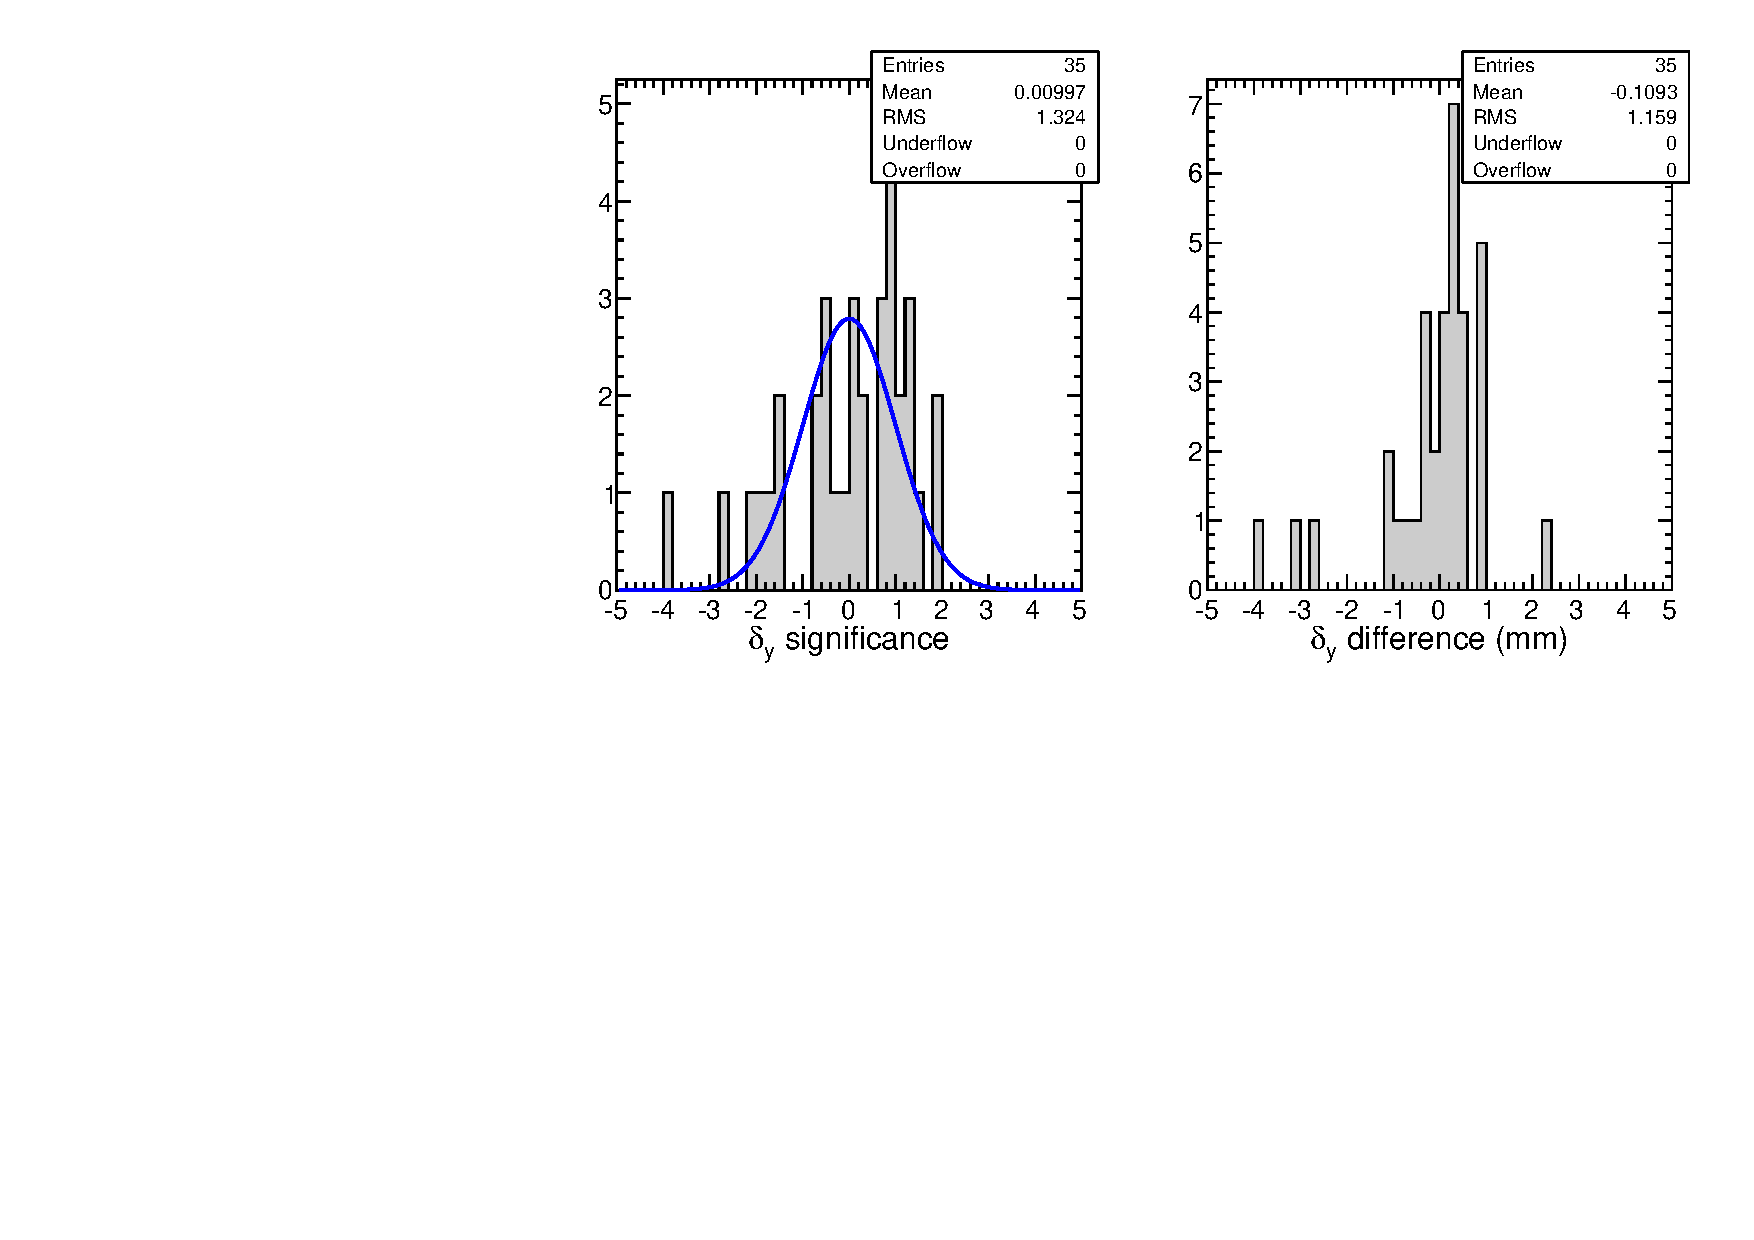
\includegraphics[width=\linewidth]{afterincident_y.pdf}
\end{frame}

\begin{frame}
\frametitle{Results (3/4)}
\begin{itemize}
\item Left: difference-over-statistical error, should be unit Gaussian

(blue curve is a unit Gaussian, not a fit)

\item Right: plain differences

\item Consistent within uncertainties: 0.6~mrad
\end{itemize}

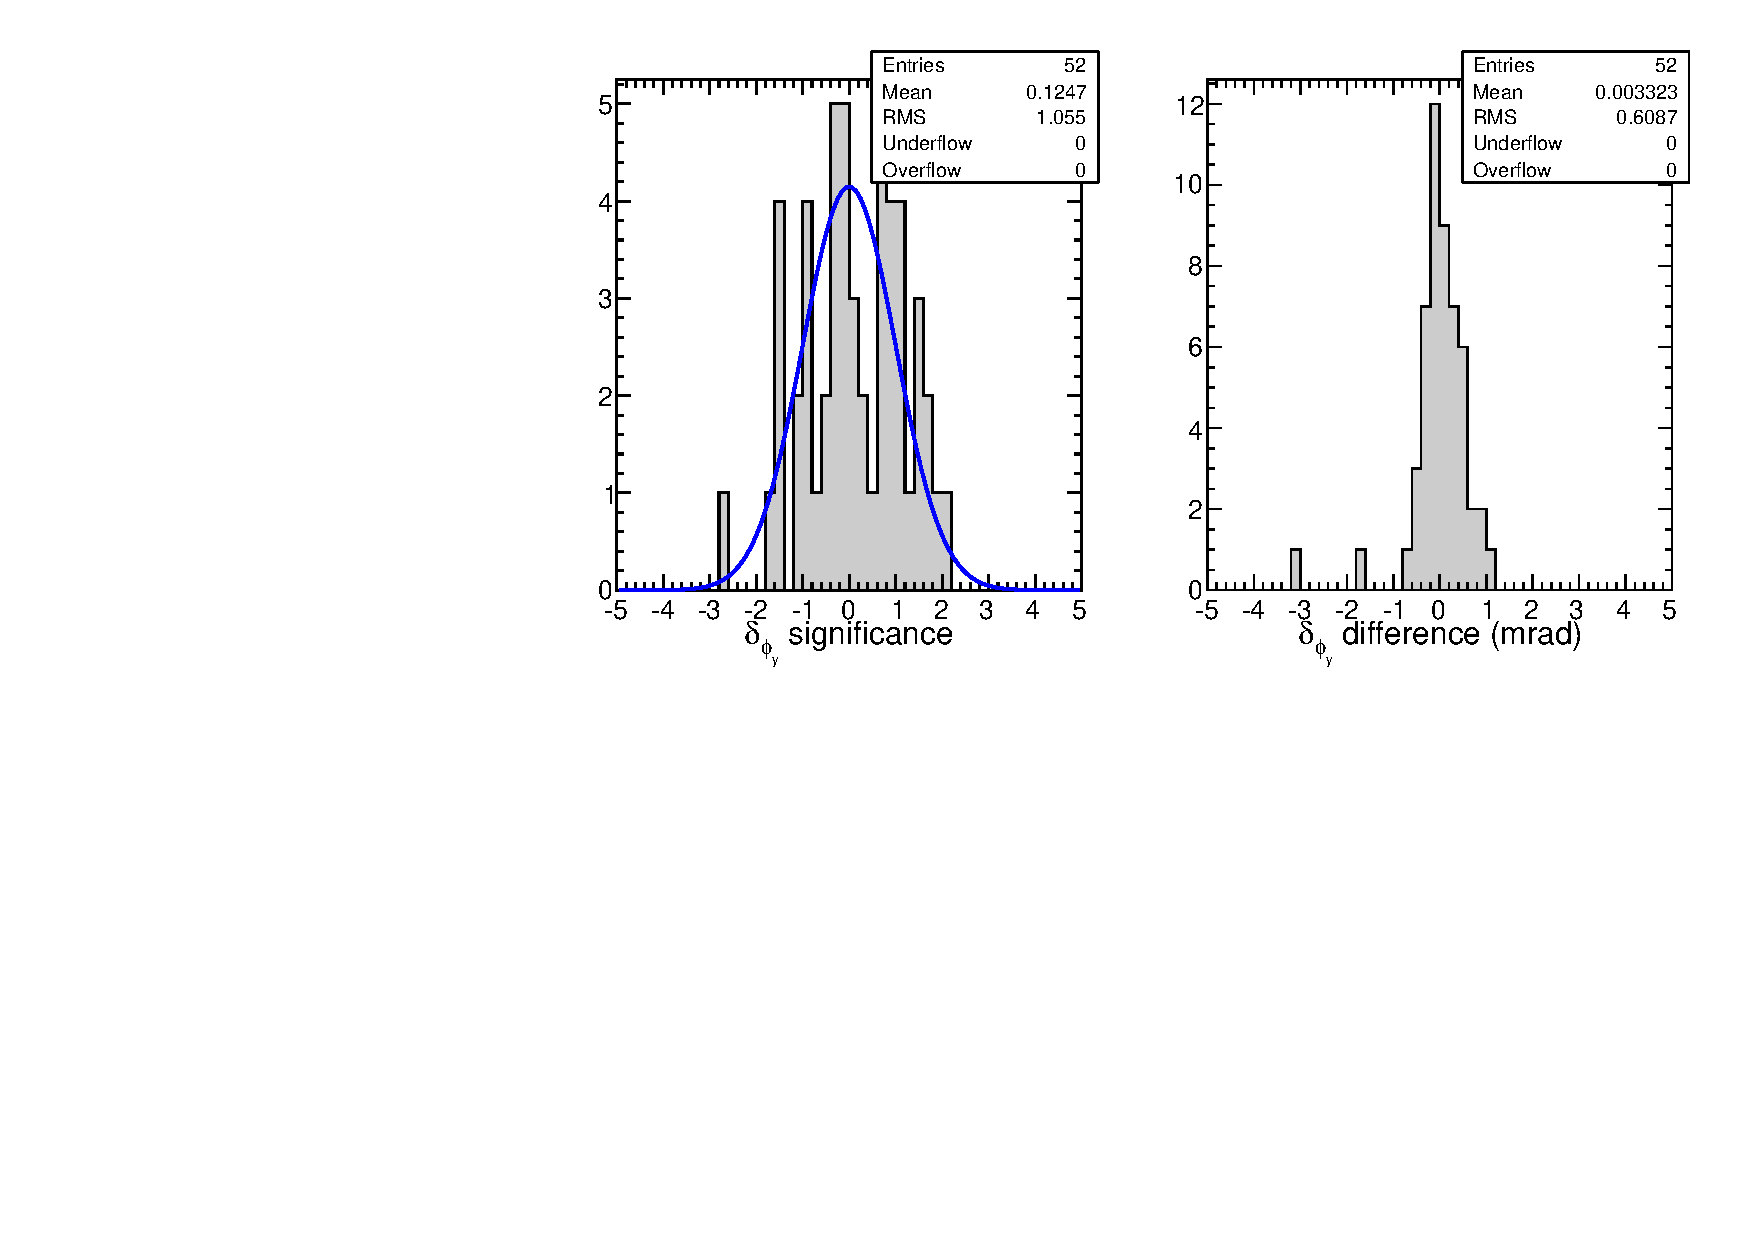
\includegraphics[width=\linewidth]{afterincident_phiy.pdf}
\end{frame}

\begin{frame}
\frametitle{Results (4/4)}
\begin{itemize}
\item Left: difference-over-statistical error, should be unit Gaussian

(blue curve is a unit Gaussian, not a fit)

\item Right: plain differences

\item Consistent within uncertainties: 1.0~mrad
\end{itemize}

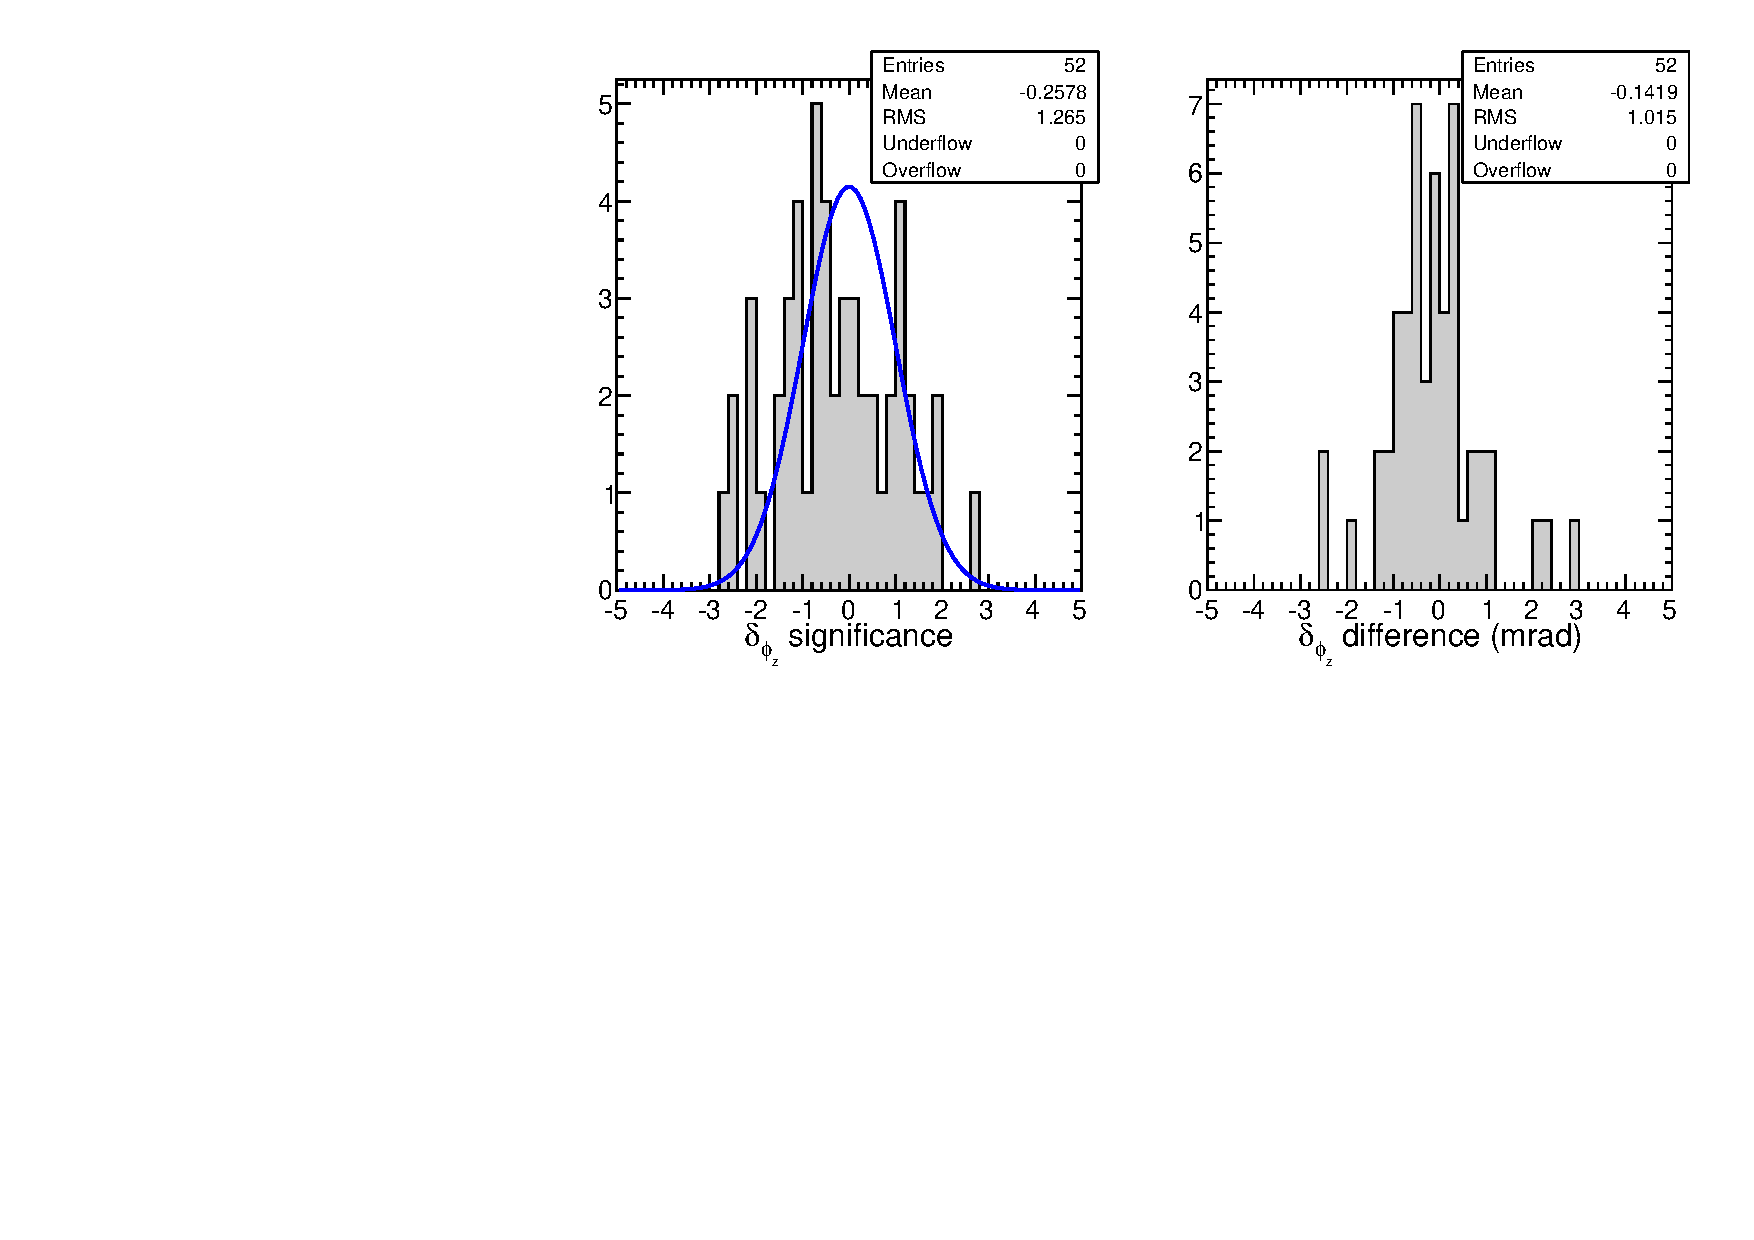
\includegraphics[width=\linewidth]{afterincident_phiz.pdf}
\end{frame}

\begin{frame}
\frametitle{DT conclusion}

\begin{itemize}\setlength{\itemsep}{0.5 cm}
\item As far as we can tell, CRAFT-09 alignment is as consistent with
  the new tracker as it was with the old tracker

\item Statistical uncertainty in this statement is 0.66~mm in $\delta_x$

\item (CRAFT-09 systematic uncertainty $\sim$ 0.35~mm in $\delta_x$,
  with much, much smaller statistical uncertainties)
\end{itemize}
\end{frame}

\begin{frame}
\frametitle{CSC beam-halo}

\begin{itemize}
\item Still very few beam-halo (lots of cosmics)

\item As of yesterday evening, still the only 121964 and 122294 (Nov~23) are
  the only beam-halo enriched runs in Prompt RECO

\item Left: identifying beam-halo enriched runs

\item Right: overlaps hits from beam-halo enriched runs
\end{itemize}

\mbox{\hspace{-1 cm}
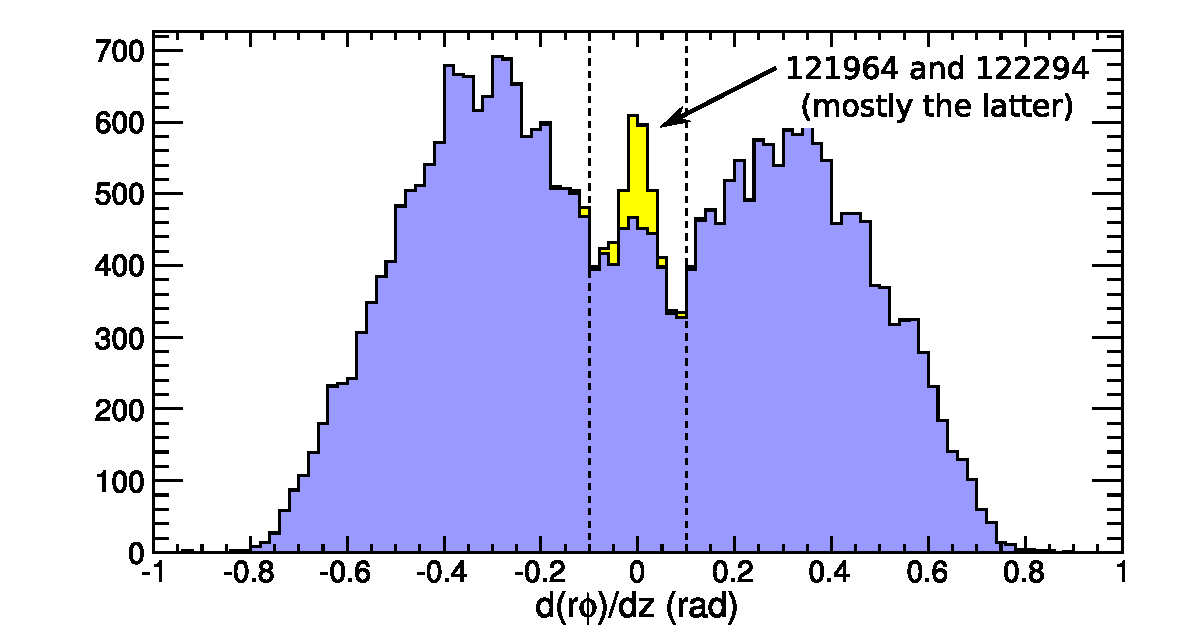
\includegraphics[height=4 cm]{beamhalo_fraction.pdf}
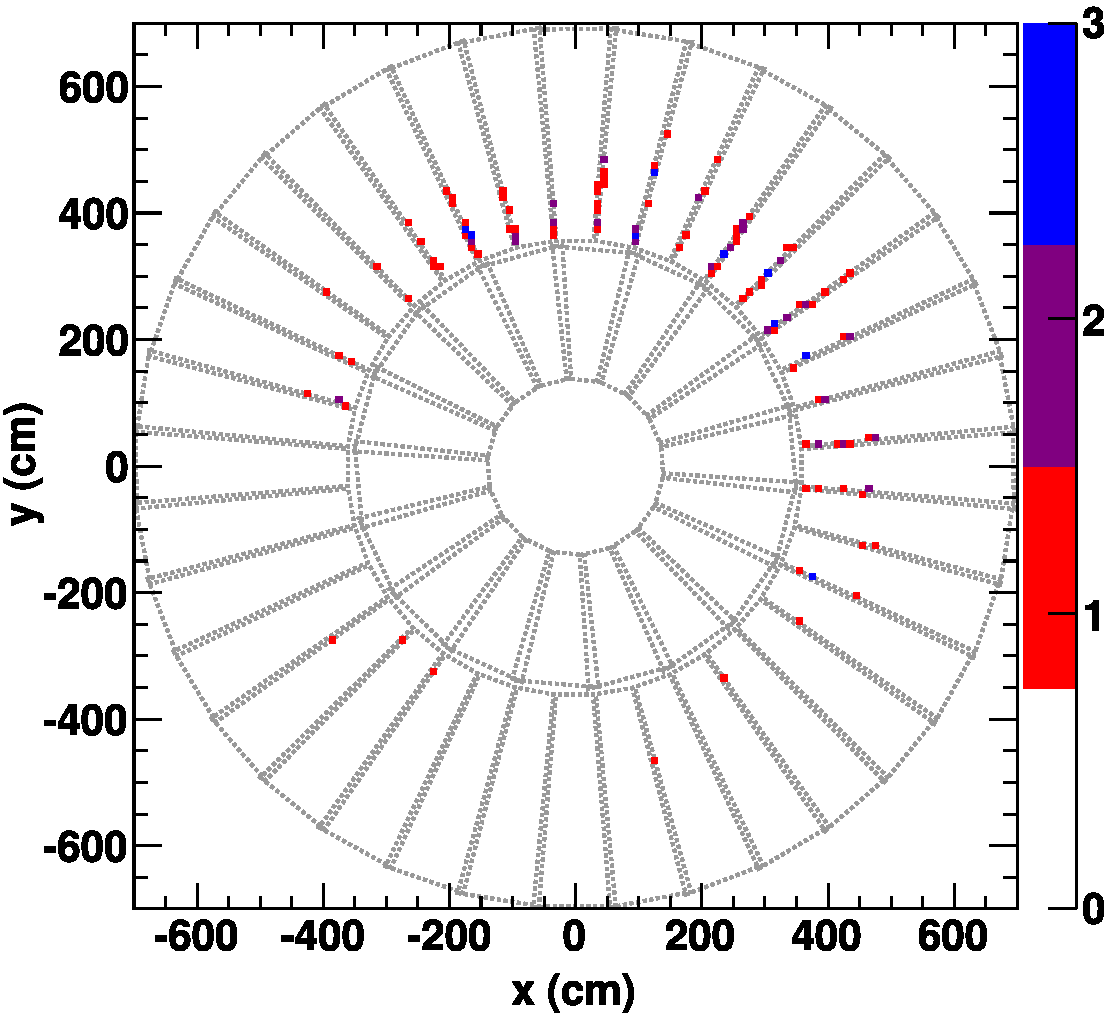
\includegraphics[height=4 cm]{xyoccupancy.pdf}}
\end{frame}


%% \begin{frame}
%% \frametitle{Outline}
%% \begin{itemize}\setlength{\itemsep}{0.75 cm}
%% \item 
%% \end{itemize}
%% %% \hspace{-0.83 cm} \textcolor{darkblue}{\Large Outline2}
%% \end{frame}

%% \section*{First section}
%% \begin{frame}
%% \begin{center}
%% \Huge \textcolor{blue}{First section}
%% \end{center}
%% \end{frame}

\begin{frame}
\frametitle{Conclusions}

\begin{itemize}
\item No proposed track-based alignment updates for early data
  re-reconstruction (Dec~17)
\end{itemize}

\label{numpages}
\end{frame}

\end{document}
